\section{Modelos Spark ML}

\subsection{Preparacion de variables}

Los modelos se entrenaron sobre \texttt{emisiones.json}. Para regresion se usaron ocho variables explicativas: \texttt{PERIODO}, \texttt{PORCENTAJE\_CONDOMINIO}, montos de parques, residuos y barrido, y descuentos/topes seleccionados. La variable objetivo fue \texttt{MONTO\_SERENAZGO}.

Para clasificacion se construyo la etiqueta \texttt{TIPO\_PREDIO}: \textit{Exclusivo} cuando \texttt{PORCENTAJE\_CONDOMINIO = 100} y \textit{Compartido} en los demas casos. Esta columna no se uso como feature en clasificacion, porque incluirla generaria fuga de datos: el modelo aprenderia directamente el umbral que define la etiqueta.

En ambos casos se aplico division entrenamiento/prueba de 80/20 con semilla fija y normalizacion de variables mediante \texttt{StandardScaler}. Por ello, las metricas no se calculan sobre los mismos registros usados para entrenar, sino sobre una particion de prueba; esto permite hablar de capacidad predictiva bajo condiciones similares a las observadas en el dataset.

\subsection{Regresion}

El enunciado solicita una regresion con Multilayer Perceptron y otra basada en maquinas de soporte vectorial. Spark MLlib no incluye de forma directa un MLP de regresion ni un SVR equivalente para regresion, por lo que ambos fueron derivados manualmente:

\begin{itemize}
    \item \textbf{MLPRegressor}: red con una capa oculta de 16 neuronas, activacion \texttt{tanh}, salida lineal y perdida MSE. El entrenamiento distribuye el calculo del gradiente mediante \texttt{treeAggregate}.
    \item \textbf{SVRegressor}: regresion de soporte vectorial lineal con perdida epsilon-insensitiva y regularizacion L2. Tambien usa agregacion distribuida de subgradientes.
\end{itemize}

\subsection{Clasificacion}

Para clasificacion se utilizaron algoritmos disponibles en Spark MLlib:

\begin{itemize}
    \item \textbf{Random Forest}: 100 arboles y profundidad maxima 8.
    \item \textbf{Multilayer Perceptron Classifier}: arquitectura \texttt{[7, 8, 4, 2]} con 200 iteraciones.
\end{itemize}

\subsection{Curvas de perdida}

Las curvas de perdida se generaron para los dos modelos derivados de regresion, porque en ellos el entrenamiento iterativo se implemento manualmente. Random Forest no expone una curva de perdida por epoca y \texttt{MultilayerPerceptronClassifier} usa optimizacion interna de Spark sin historial exportado equivalente.

\begin{figure}[H]
    \centering
    \begin{subfigure}{0.49\textwidth}
        \centering
        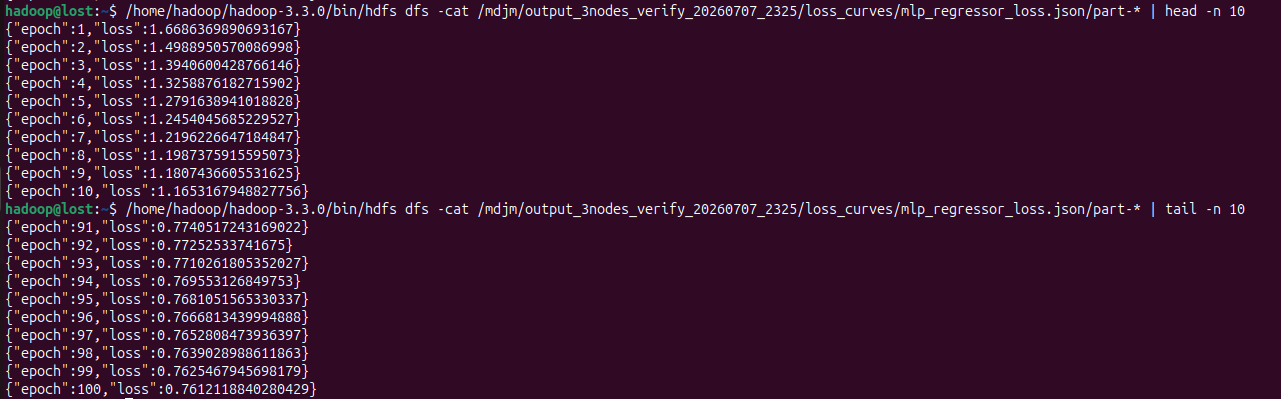
\includegraphics[width=\textwidth]{ImgNod1/Curva_Perdida_MLP_Regre.png}
        \caption{MLPRegressor.}
    \end{subfigure}
    \begin{subfigure}{0.49\textwidth}
        \centering
        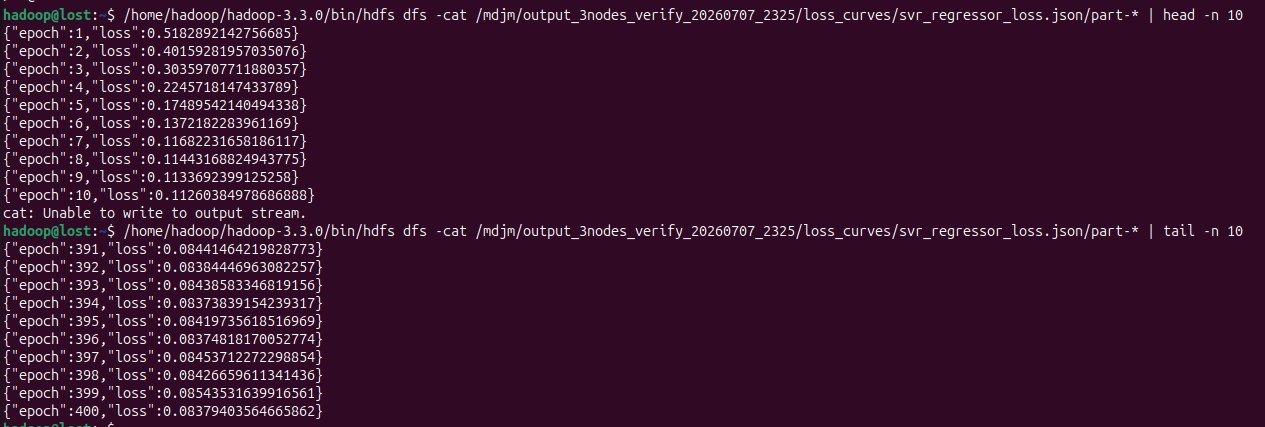
\includegraphics[width=\textwidth]{ImgNod1/Curva_Perdida_svr_regresor.png}
        \caption{SVRegressor.}
    \end{subfigure}
    \caption{Curvas de perdida de entrenamiento para los modelos de regresion derivados.}
    \label{fig:loss-curves}
\end{figure}
